% Supervisor meeting brief. Build: tectonic meeting_brief.tex
\documentclass[11pt,a4paper]{article}

\usepackage[margin=2.4cm]{geometry}
\usepackage{graphicx}
\usepackage{booktabs}
\usepackage{float}
\usepackage{caption}
\usepackage{enumitem}
\usepackage{microtype}
\usepackage{newtxtext,newtxmath}
\usepackage[hidelinks,pdfauthor={Luca Wuerker},
            pdftitle={Ablation Results and Final Experiment}]{hyperref}

\captionsetup{font=small,labelfont=bf,width=.95\textwidth}
\setlist{itemsep=2pt,topsep=3pt}

\title{\bfseries Ablation Results \& Final Experiment}
\author{Luca W\"urker}
\date{August 2026}

\begin{document}
\maketitle

\noindent\textbf{Protocol.} Nasdaq-100 point-in-time panel, 2010--2026,
survivorship-bias-free. Research uses data to mid-2021; 2021--26 is consumed
as ten six-month blocks, each scored \emph{before} the researcher may adapt
to it --- a five-year honest walk-forward record per run. All numbers are
signal-level ICs; no position construction or costs.

\medskip
\noindent\textbf{Baseline.} The full configuration: LLM ideation grounded in
a knowledge graph of 1{,}723 papers (eight mechanism communities), candidates
compiled and scored by a deterministic harness on four objectives (marginal
value to the book, independence, parsimony, structural novelty), twenty
generations of LLM mutation/crossover under progressive data reveal. 57
factors, $\sim$900 scored candidates, \$250. Each arm below removes or adds
one ingredient; everything else is held fixed.

\begin{figure}[H]\centering
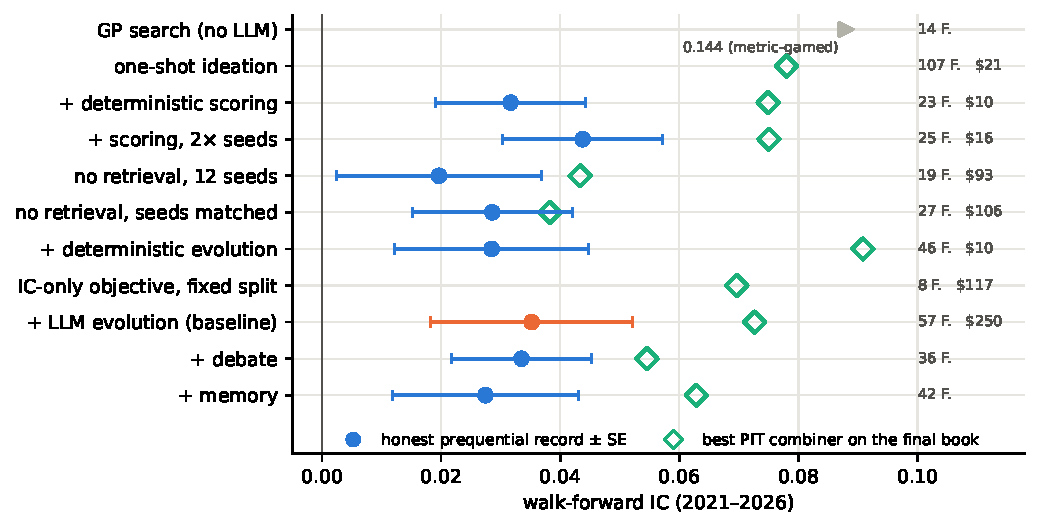
\includegraphics[width=.92\textwidth]{figures2/l1_ladder}
\caption{The ablation ladder. Dots: honest walk-forward record (mean of the
ten block ICs $\pm$ SE). Diamonds: best point-in-time combiner applied to
the arm's final book. Right margin: book size and LLM cost.}
\end{figure}

\begin{table}[H]\centering\small
\begin{tabular}{llccccc}
\toprule
Arm & Candidate evaluation & WF IC & PIT best & Book & Cost \\
\midrule
GP (no LLM)        & 4-axis, incremental        & 0.144\,* & ---   & 14  & \$0   \\
One-shot           & none --- keep all          & ---      & 0.078 & 107 & \$21  \\
+ det.\ scoring    & 4-axis at admission        & +0.032   & 0.075 & 23  & \$10  \\
+ scoring, 2$\times$ seeds & 4-axis at admission & \textbf{+0.044} & 0.075 & 25 & \$16 \\
No retrieval (96 seeds) & 4-axis + reveal       & +0.029   & 0.038 & 27  & \$106 \\
+ det.\ evolution  & 4-axis + reveal            & +0.028   & \textbf{0.091} & 46 & \$10 \\
IC-only, fixed split & $|$VAL IC$|$ only        & ---      & 0.070 & 8   & \$117 \\
Full LLM evolution & 4-axis + reveal            & +0.035   & 0.073 & 57  & \$250 \\
+ debate           & 4-axis (indep.\ axis inactive) & +0.033 & 0.055 & 36 & ---  \\
+ memory           & 4-axis (indep.\ axis inactive) & +0.027 & 0.063 & 42 & \$206 \\
\bottomrule
\end{tabular}
\caption{* metric-gamed (integrated price/fundamental levels), not alpha.
Block SE $\approx$ 0.012--0.019. ``One-shot'' keeps every factor that
compiles; the scoring arms evaluate each seed on the four objectives
sequentially at admission (against the book built so far) and then re-score,
prune and curate for twenty generations without generating children.}
\end{table}

\begin{figure}[H]\centering
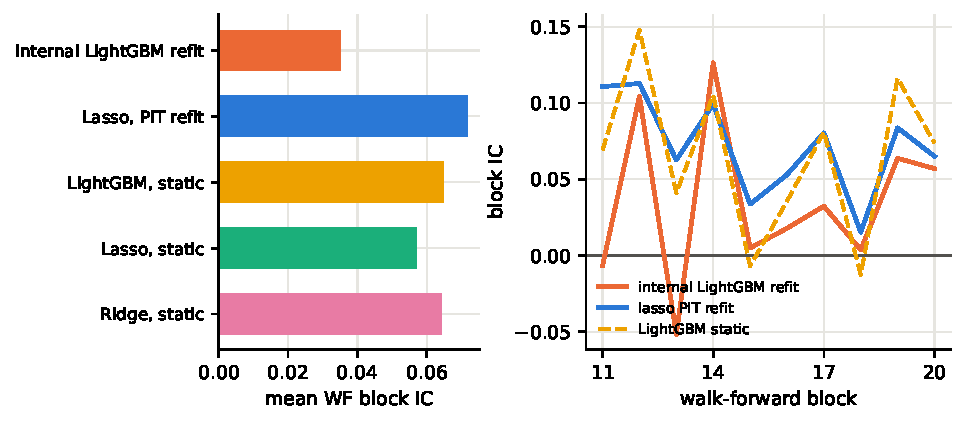
\includegraphics[width=.95\textwidth]{figures2/b2_l4_combiners}
\caption{Baseline book, five ways to combine it. The prequential LightGBM
refit the search optimises against (orange) is the weakest deployment
combiner; a point-in-time lasso refit doubles it and is positive in every
block. The same ordering holds in every arm.}
\end{figure}

\begin{figure}[H]\centering
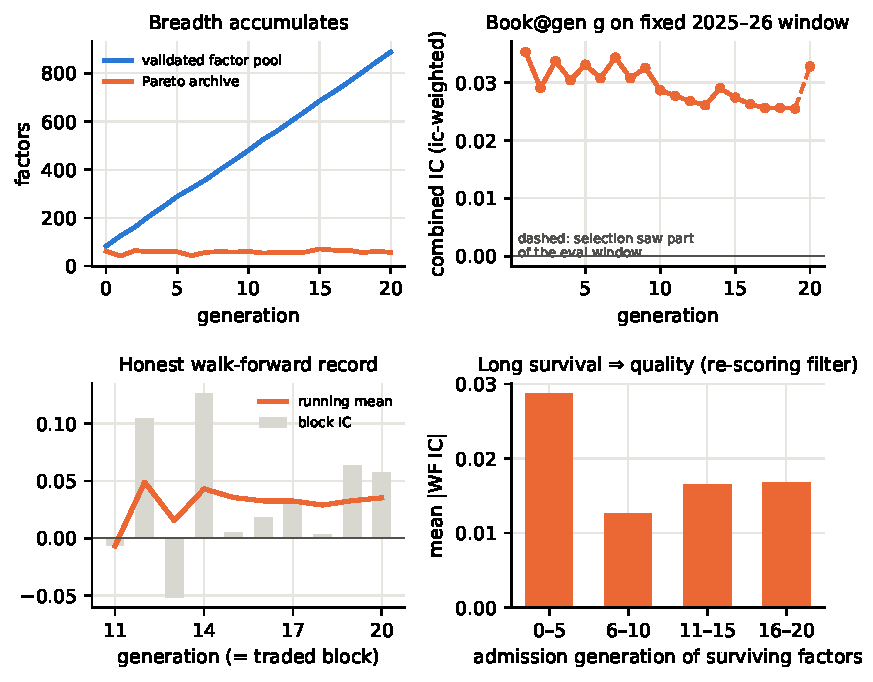
\includegraphics[width=.95\textwidth]{figures2/l3_learning}
\caption{What actually changes over the evolution (baseline). Breadth
accumulates (pool 83$\to$890) while the archive holds at its cap; the
archive as of each generation, recombined identically on a fixed 2025--26
window, is flat --- the generation-1 book was already as good; the honest
record stabilises at $\approx+0.035$; and the earliest admits --- re-scored
up to twenty times on growing, partly unseen windows --- carry twice the
realised $|$IC$|$ of later cohorts.}
\end{figure}

\section*{Takeaways}
\begin{enumerate}
\item \textbf{Per-factor edge transfers out of sample.} Fit-window versus
walk-forward per-factor IC: retention $r=0.94$, only 18\% of baseline
factors flip sign, mean $|$IC$|$ unchanged (0.019 $\to$ 0.018). The
\emph{combiner} is the fragile part: point-in-time linear recombination
doubles the internal boosted-tree score (0.073 vs.\ 0.035) --- so results
should be reported combiner-robust, not on one combiner's IC.
\item \textbf{Ideation + deterministic scoring carries the record.} Seeding
once and letting the harness score, prune and curate --- no evolution ---
matches the \$250 full-evolution record at \$10--16; doubling the seed
budget gives the family's best honest record ($+0.044$). In-loop LLM
mutation, debate and cross-run memory add nothing measurable.
\item \textbf{Every naive objective gets gamed.} The prior-free GP maximises
its reward with integrated price/fundamental levels and, after a targeted
stationarity gate, evades it with near-boundary proxies (Goodhart). Scoring
by validation IC alone on a fixed split shows textbook winner's curse:
promised median $|$IC$|$ 0.040 $\to$ 0.025 delivered, five of eight
survivors sign-unstable, the archive collapsed to one factor per group.
Multi-objective selection + progressive reveal are what make individual
factors trustworthy.
\item \textbf{Retrieval grounding doubles deployable value, not the
headline.} With seeding matched, the no-retrieval arm ties the baseline's
record ($+0.029$ vs.\ $+0.035$) but produces the family's weakest factors
(median $|$IC$|$ 0.005, 44\% sign flips, lowest effective dimension) and
recombines to 0.038 versus 0.073. (The first no-retrieval runs were
confounded --- underseeded by a since-fixed timeout bug; the control run
resolves it.)
\item \textbf{Evolution buys breadth and sign stability, not mean IC.} The
generation-1 book already scores as well on a fixed future window as any
later one; survival through repeated re-scoring is the effective quality
filter. Deterministic jitter evolution captures this cheaply: the best
point-in-time book of the family (0.091) at \$10.
\item \textbf{All results are single-seed; differences within $\pm$0.01 are
noise.} This motivates the design of the final experiment.
\end{enumerate}

\section*{Final experiment: LLM comparison}
Last remaining study: several research LLMs on one fixed configuration.
Chosen configuration: \textbf{grounded ideation + deterministic scoring} ---
192 graph-grounded seed ideas (24 per mechanism community), no evolutionary
children, the full walk-forward scoring machinery; the knowledge graph is
frozen so every model sees identical context; arms are seed-matched, with
realised cost reported as a secondary result.

\begin{itemize}
\item \textbf{It isolates what varies between models} --- idea quality and
code quality --- judged by a fixed deterministic harness. Full evolution
would spend most of each budget on machinery the ablations show adds
nothing, diluting the model contrast with selection noise.
\item \textbf{It is the family's efficient frontier}: best honest record
($+0.044$) and point-in-time 0.075, on par with the \$250 baseline.
\item \textbf{Statistical power per dollar}: $\sim$\$20 per run allows two
to three seeds per model --- roughly \$250 for six models, the price of one
full-evolution run --- addressing the single-seed weakness directly.
\item \textbf{Everything downstream exists}: reference runs on the current
model, and the standardised evaluation (prequential record, combiner race,
per-factor $|$IC$|$, sign stability, effective dimension) applies unchanged.
\end{itemize}

\noindent Planned comparisons: the current reference model plus
frontier-class and mid-tier alternatives from the major providers, two seeds
each; identical prompts, graph snapshot, budget cap per arm. Metrics: honest
walk-forward record, best-combiner book IC, factor validity rate, per-factor
$|$IC$|$ and sign stability, diversity, and cost per validated factor.
Before launch: fix the coverage bug that silently disabled the independence
objective in the debate arms.

\end{document}
